\documentclass[12pt]{article}
\usepackage{../eplcrypto}
\usepackage{geometry} % see geometry.pdf on how to lay out the page. There's lots.
\geometry{a4paper} % or letter or a5paper or ... etc
% \geometry{landscape} % rotated page geometry
\usepackage[parfill]{parskip}
% See the ``Article customise'' template for come common customisations
\usepackage{amsmath}
\usepackage{graphicx}
\usepackage{amssymb}
\usepackage{algorithmic}
\usepackage{algorithm}
\title{Slides04}

%%% BEGIN DOCUMENT
\begin{document}

\maketitle
\tableofcontents
\newpage

\section{Message Authenticity}
In the course so far we have only considered confidentiality aspect of communication. Message authenticity is an important aspect as well. The questions of "does this message really come from the person I am expecting from?" and "Am I sure that is has not been modified?" are also important.

It is possible that the attacker manages to flip one bit and the message is completely different now than what was intended. This could be that it is a transaction and the attacker know which part of the ciphertext contains the money and even though he cannot know what is inside the ciphertext, he can still change one bit to change the sum that is being transferred from one account to another.

\subsection{Authenticity}
There are two flavours of authenticity:
\begin{description}
\item[\quad 1. Integrity:] Is this message authentic?
\item [\quad 2. Non malleability:] Could this plaintext result from a controlled manipulation of a ciphertext.
\end{description}

The goal is to make the modificaitons to the ciphertext detectable.

\section{Message Authentication codes (MAC)}
\subsection{Principle}
To perform authenticated communication.
\begin{itemize}
\item Alice and Bob agree on a common key k
\item To send message m, Alice does
	\begin{itemize}
	\item Uses a generation algorithm to compute a tag $t$ from $m$ and $k$
	\item Sends $m$ together with $t$
	\end{itemize}
\item On reception of $(m,t)$
	\begin{itemize}
	\item Uses a verification algorithm to check whether $t$ is a valid tag for $m$ and $k$
	\item Accepts $m$ iff the answer is positive.
	\end{itemize}
\end{itemize}
\newpage
\subsection{Definition}
A message authentication code is a triple $\Pi \define \langle \Gen, \Mac, \Vrfy \rangle$
\begin{itemize}
\item $\Gen$: Probabilistically selects a key $k \in \K$
\item $\Mac$: On input $m \in \M$ and $k \in \K$ computes a tag $t\leftarrow \Mac_k(m)$
\item $\Vrfy$: On input $m,t,k$ outputs a bit $b \define \Vrfy_k(m,t)$, with $b=1$ meaning valid, $b=0$ meaning invalid
\end{itemize}

Remarks:
\begin{itemize}
\item Probabilistic encryption is mandatory for CPA-security.
\item Mac \emph{may} be probabilistic (having same tags is not a problem)
\item $\Vrfy$ is deterministic. 
\end{itemize}

\subsubsection{MAC correctness}
$\forall m \in \M$ and $\forall k \in \K$, it must hold that:
\begin{equation*}
\Vrfy_k(m,\Mac_k(m))=1
\end{equation*}

\subsubsection{MAC security}
\textbf{Intuition}: No PPT adversary should be able to generate a valid tag on any "new" message. Even if adversary can observe valid MAC tags and could obtain valid MAC tags for messages that he chooses (oracle model).

\subsubsection{Experiment: $\MacForge_{\A,\Pi}(n)$}
Given $\Pi \define \langle \Gen, \Mac, \Vrfy \rangle$, and an adversary $\A$, define the following experiment $\MacForge_{\A,\Pi}(n)$:
\begin{enumerate}
\item Choose $k\leftarrow Gen(1^n)$
\item $\A$ is given oracle access to $\Mac_k(\cdot)$. Let $\Q$ denote the set of queries made to $\Mac_k(\cdot)$
\item $\A$ outputs a pair $(m,t)$
\item Define $\MacForge_{\A,\Pi}(n) \define 1$ iff $\Vrfy_k(m,t)=1$ and $m \notin \Q$
\end{enumerate}
\newpage
$\Pi \define \langle \Gen, \Mac, \Vrfy \rangle$ is \emph{existentially unforgeable under an adaptive chosen-message attack} (EUF-CMA) if $\forall$ PPT $\A$, $\exists\,\negl$:
\begin{equation*}
Pr[\MacForge_{\A,\Pi}(n)] \le \negl(n)
\end{equation*}

\subsubsection{More on EUF-CMA security}
\textbf{Existential attacks:} $\A$ wins if he forges anything, even some meaningless messages.
Even though this existential attack inclusion makes MAC application independent, it still does not protect from replay attacks (repeat send \$100 from a bank).\\
Need challenge response or time-stamping type of solutions.

\subsubsection*{Quiz}
\begin{itemize}
\item Suppose $\A$ submits $m$, gets $t$ and then outputs $(m',t)$ such that $m\neq m'$ and $\Vrfy(m',t)=1$\\
\quad $==>$This is an attack
\item Suppose $\A$ submits $m$, gets $t$ and then outputs $(m,t')$ such that $t\neq t'$ and $\Vrfy(m,t')=1$\\
This is not a problem, "no PPT adversary should be able to generate a valid tag on any ”new” message".
\end{itemize}

Notion of \emph{strong} unforgeability:
\begin{itemize}
\item A stronger notion than EUF-CMA
\item $\A$ wins as soon as he produces new valid $(m,t)$ pair
\end{itemize}

\subsection{Constructing secure MACs}
We will use pseudorandom functions.

Define $\Pi \define \langle \Gen, \Mac, \Vrfy \rangle$ as:
\begin{itemize}
\item $\Gen$: Choose random $k\leftarrow \zo^n$
\item $\Mac$: On input $m,k \in \zo^n$, output $t \define F_k(m)$
\item $\Vrfy$: On input  $m,k,t \in \zo^n$ output 1 iff $t = F_k(m)$
\end{itemize}
\newpage
\subsubsection{Security of PRF-based MAC}
\textbf{Theorem:} If $F$ is a PRF, this MAC is EUF-CMA secure.\\
\textbf{Proof:} In two steps
\begin{itemize}
\item Prove that the scheme is secure if $F_k$ is replaced by a truly random function $f$
\item Prove that if the scheme (with $F_k$) were insecure, we could distinguish $F_k$ from a truly random function.
\end{itemize}
 This is very similar to the CPA-security proof.\\
 We construct a polynomial-time distinguisher $D$ that is given oracle access to some function $\O$ and whose goal is to determine whether $\O$ is pseudorandom($F_k$) or random ($f$).
 
 So what we do here is to ask the question of can we use the MAC construction we came up with as a subroutine for a distinguisher $D$. To do this, D simulates the message authentication experiment for $\A$ and observes whether $\A$ succeeds in outputting a valid tag on a “new” message. If so, $D$ guesses that its oracle is a pseudorandom function; otherwise, $D$ guesses that its oracle is a random function.
Proof in the section 4.3.1 of the book.

\subsection{Extension to variable-length messages}
It is possible to construct a MAC handling arbitrary length messages from any fixed-length MAC for messages of length $n$.\\
As $F_k$ is a length-preserving function, our construction only works for messages such that $|m|=|k|$.\\
Consider now $m=m_1||\dots||m_d$ such that $|m_i|=|k|$

\begin{enumerate}
\item $t_i \define \Mac_k'(m_i)$ and output $\langle t_1,\dots,t_d\rangle$. This prevents an adversary from sending any previously unauthenticated block without being detected. However, it does not prevent a "block re-ordering attack" in which the attacker shuffles the order of blocks in an unauthenticated message. If $\langle t_1, t_2\rangle$ is a valid tag on message $m_1,m_2$, with $m_1 \neq m_2$, then an attacker can construct a valid tag $\langle t_2, t_1\rangle$ on the (new) message $m_2, m_1$. Something that is not allowed in our definition of secure MAC.

\item Prevent the "block re-ordering attack" by $t_i \define \Mac_k'(i||m_i)$ for all $i$ and output $\langle t_1,\dots,t_d\rangle$ as the tag. This does not prevent a truncation attack whereby an attacker simply drops blocks from the end of the message (and drops the corresponding blocks of the tag as well).

\item A truncation attack can be thwarted by additionally authenticating the message length along with each block.  $t_i \define \Mac_k'(l||i||m_i)$ for all $i$ where $l$ is the message length in bits. This scheme is vulnerable to a “mix-and-match” attack where the adversary combines blocks from different messages. outputting $\langle t_1, t_2' \rangle$ for $m_1, m_2'$
\end{enumerate}

We can prevent this last attack by also including a random “message identifier” in each block that prevents the attacker from combining blocks from different messages.

\begin{equation*}
t_i \define \Mac_k(r||l||i||m_i)
\end{equation*}
\begin{itemize}
\item Message block
\item Block number (to prevent block reordering)
\item Full message length (to prevent message truncation)
\item Unique, random identifier (to prevent message combination)
\end{itemize}

\subsubsection{The Construction}
Let $\Pi' = (\Mac',\Vrfy')$ be a fixed-length MAC for messages of length n\\
Define a variable-length MAC $\Pi = (\Mac,\Vrfy)$ as follows:
\begin{itemize}
\item $\Gen$: Choose random $k\leftarrow \zo^n$
\item $\Mac$: On input $k \in \zo^n$ and $m \in \zo^*$ of length $l < 2^{\frac{n}{4}}$
	\begin{itemize}
	\item Parse $m$ into blocks $m_1,\dots,m_d$ of length $\frac{n}{4}$ each (pad with 0s if necessary)
	\item Choose random $r \leftarrow \zo^{\frac{n}{4}}$
	\item Compute $t_i \define \Mac_k(r||l||i||m_i)$ for $1 \le i \le d$, with $|r|=|l|=|i|=\frac{n}{4}$
	\item Output $t\define \langle r, t_1, \dots, t_d\rangle$
	\end{itemize}
\item $\Vrfy$: On input $k,m,t = \langle r, t_1, \dots, t_d\rangle$,
	\begin{itemize}
	\item Parse $m$ into blocks $m_1,\dots,m_d$ of length $\frac{n}{4}$ each
	\item Output 1 iff $d=d'$ and, $\forall$ $1\le i\le d$, $\Vrfy_k'(r||l||i||m_i)=1$ 
	\end{itemize}
\end{itemize}
\textbf{Theorem:} If $\Pi'$ is secure fixed-length MAC for messages of length n, then $\Pi$ is a MAC that is existentially unforgeable under an adaptive chosen-message attack.
\textbf{Proof}: By reduction. Any adversary breaking $\Pi$ can be turned into an adversary breaking $\Pi'$.

\subsection{CBC-MAC}
A construction similar to the CBC mode of encryption. Probably secure. Efficient:
\begin{itemize}
\item For a d-block message, d executions of the PRF
\item Tag is 1 block long
\end{itemize}

\begin{figure}[ht]
    \centering
    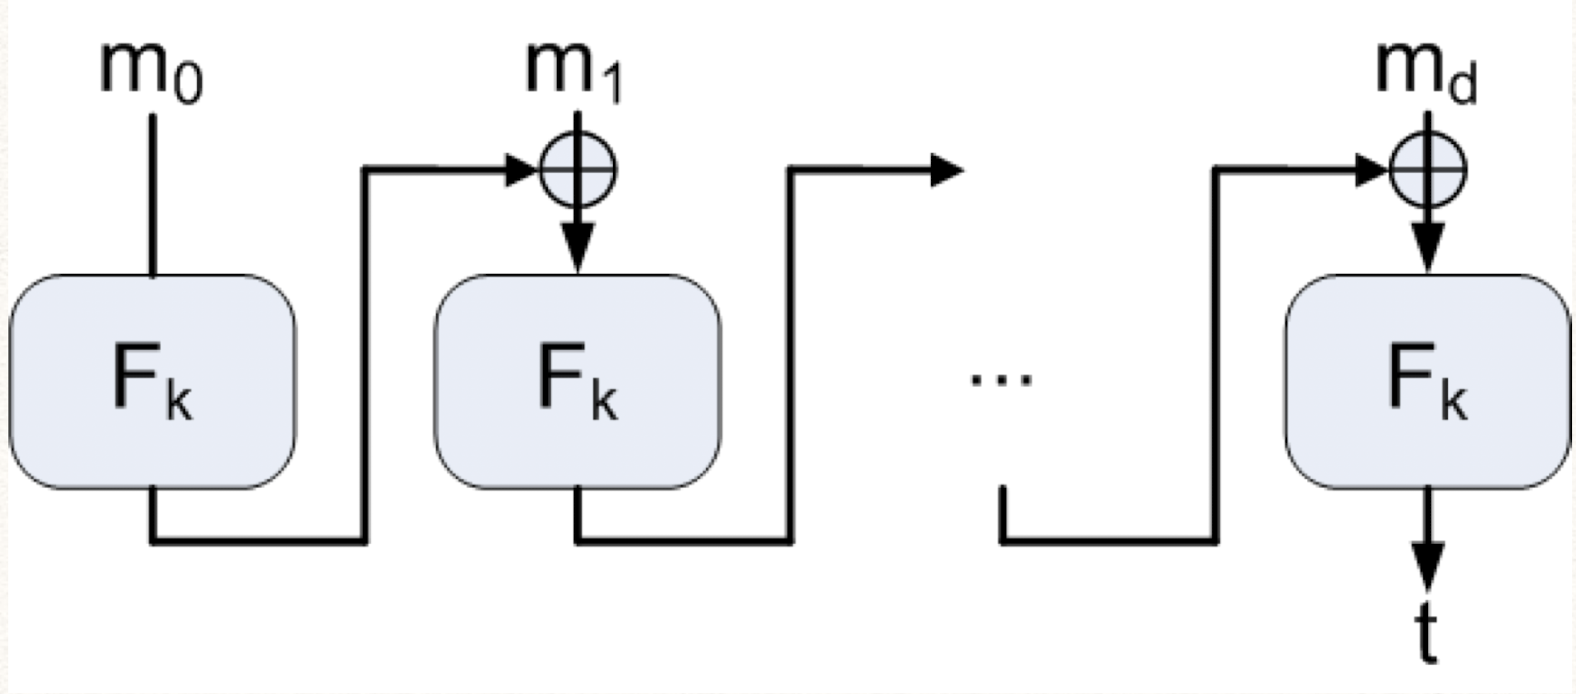
\includegraphics[width=12cm]{figures/f1.png}
\end{figure}
Remark: If intermediary values are output, scheme is not secure any more!

\textbf{Theorem:} \emph{If $F$ is a PRF, then CBC-MAC is a fixed length MAC that is existentially unforgeable under an adaptive chosen-message attack.}

This scheme is not secure for variable-length messages.

\subsubsection{CBC-MAC for variable-length messages}

\begin{figure}[ht]
    \centering
    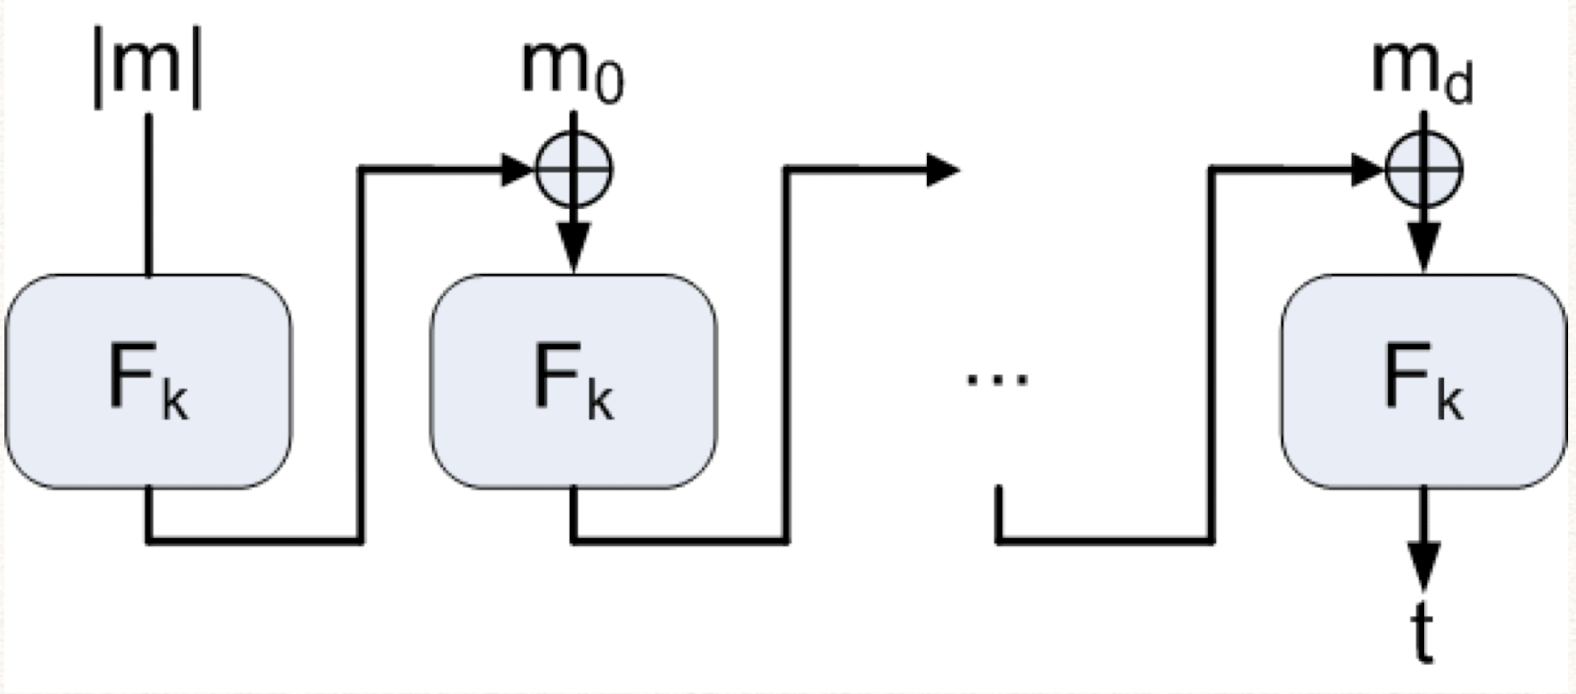
\includegraphics[width=12cm]{figures/f2.png}
\end{figure}
This construction is provably secure, but with complex proof.
\newpage
\subsection{Summary: What can and cannot be done with a MAC?}
MACs allow:\begin{itemize}
\item Reliable exchange of information between parties having agreed on a key and trusting each other 
\end{itemize}

But anyone who can check a MAC can also forge one, which makes it suitable only for "closed communities" where the symmetric key can be shared.



\section{Authenticity}
There are two flavours of authenticity:
\begin{description}
\item[\quad 1. Integrity:] Is this message authentic?
\item [\quad 2. Non malleability:] Could this plaintext result from a controlled manipulation of a ciphertext.
\end{description}
\subsubsection*{Is CPA security a sufficient criterion?}
We have given the adversary the possibility to:
\begin{itemize}
\item Observe ciphertexts
\item Encrypt plaintexts of his choice
\end{itemize}
What else an attacker could do?
\begin{itemize}
\item Decrypt ciphertexts of his choice
\end{itemize}
\textbf{We will formalize this by giving $\A$ access to a decryption oracle.}
\newpage


\subsection{Chosen-Ciphertext Attacks (CCA)}
\subsubsection{Experiment: $\PrivKcca$}
Given $\Pi \define \langle \Gen, \Enc, \Dec \rangle$, and adversary $\A$, define the following as the experiment:
\begin{enumerate}
\item Choose $k \leftarrow \Gen(1^n)$
\item $\A$ is given oracle access to $\Enc_k(\cdot)$ and $\Dec_k(\cdot)$
\item $\A$ outputs $m_0,m_1 \in \M$
\item Choose $b\leftarrow \zo$ and send $c\define\Enc_k(m_b) $ to $\A$
\item $\A$ is again given oracle access to $\Enc_k(\cdot)$ and $\Dec_k(\cdot)$ but cannot ask $\Dec_k(c)$
\item $\A$ outputs $b'$
\item Define $\PrivKcca(n)\define 1$ iff $b=b'$
\end{enumerate}

$\Pi \define \langle \Gen, \Enc, \Dec \rangle$ has indistinguishable encryption under a chosen-ciphertext attack if $\forall$ PPT $\A$, $\exists\,\negl$:
\begin{equation*}
Pr[\PrivKcca(n)=1] \le \frac12 + \negl(n)
\end{equation*}

\subsubsection{Security against CCA}
\emph{None of the schemes we saw so far is CCA-secure!}\\
\textbf{Example:} Attacking the scheme $c\define \langle r,F_k(r)\xor m \rangle$
\begin{itemize}
\item Send $m_0 = 0^n, m_1=1^n$ and receive $c\define Enc_k(m_b)$
\item Flip the last bit of c
\item Ask the decryption of flipped message
\item See whether you get $0\dots01$ or $1\dots10$
\end{itemize}
As long as $\A$ can manipulate ciphertexts, we cannot prevent this kind of attack.
\textbf{CCA is good enough in many cases:}
\begin{itemize}
\item Encrypt a key: Any manipulation will results in an unrelated key, that will not work and can be leaked without risk
\item Encrypt a vote: Any vote manipulation will result in an unrelated vote, that cannot leak about the original one
\end{itemize}
\newpage
\textbf{Unforgeable ciphertexts:}
\begin{itemize}
\item If decryption succeeds, then I have the right key
\item If vote is valid, then it contains the expected intent
\end{itemize}

\subsection{Unforgeable Encryption}
\subsubsection{Experiment: $\EncForge(n)$}
Given $\Pi \define \langle \Gen, \Enc, \Dec \rangle$, and an adversary $\A$ define the following experiment $\EncForge(n)$:
\begin{enumerate}
\item Choose $k\leftarrow \Gen(1^n)$
\item $\A$ is given oracle access to $\Enc_k(\cdot)$, all queries of $\A$ is stored in $\Q$
\item $\A$ outputs $c$
\item Define $\EncForge(n) \define 1$ iff $(\Dec_k(c) \neq \perp$ and $\Dec_k(c)  \notin \Q)$
\end{enumerate}
Idea: Produce a decryption of something, could you?\\
The encryption scheme $\Pi \define \langle \Gen, \Enc, \Dec \rangle$ is unforgeable if $\forall$ PPT $\A$, $\exists\,\negl$:
\begin{equation*}
Pr[\EncForge(n)=1] \le \negl(n)
\end{equation*}

\textbf{Observe:}
\begin{itemize}
\item $\Enc$ behaves like a MAC with message recovery (through $\Dec$)\\
Prevent forgery of encryption of new messages
\item Unforgeability gives authenticity, not confidentiality
\end{itemize}

\subsection{Authenticated Encryption}
$\Pi \define \langle \Gen, \Enc, \Dec \rangle$ is an authenticated encryption scheme (AE) if it is CCA-secure and unforgeable.
\newpage
\subsubsection{Experiment: $\PrivKae(n)$}
\begin{enumerate}
\item A key $k$ is generated by running $\Gen(1^n)$
\item A uniform bit $b \in \zo$ is chosen
\item The adversary $\A$ is given input $1^n$ and access to two oracles:
	\begin{enumerate}
	\item If $b=0$, then $\A$ is given access to $\Enc_k(\cdot)$ and $\Dec_k(\cdot)$
	\item If $b=1$, then $\A$ is given access to $\Enc_k^0(\cdot)$ and $\Dec_{\perp}(\cdot)$
	\end{enumerate}
	$\A$ is not allowed to query a ciphertext c to its second oracle that it previously received as the response from its first oracle.
\item The adversary outputs a bit $b'$
\item The output of the experiment is defined to be 1 if $b'=b$, and 0 otherwise. In the former case, we say that $\A$ succeeds.
\end{enumerate}
$\Pi \define \langle \Gen, \Enc, \Dec \rangle$ is an unauthenticated encryption (AE) scheme if $\forall$ PPT $\A$, $\exists\,\negl$:
\begin{equation*}
Pr[\PrivKae(n)=1] \le \frac12 + \negl(n)
\end{equation*}

\subsubsection{Combining MAC and encryption}
\begin{enumerate}
\item \emph{Encrypt-and-authenticate}: In this approach, encryption and message authentication are computed independently in parallel. 
    \begin{gather*}
        c \leftarrow \Enc_{k_E}(m) \\
        t \leftarrow \Mac_{k_M}(m)
    \end{gather*}
    The receiver decrypts $c$ to recover $m$; assuming no error occurred, it then verifies the tag $t$.\\
\textbf{Remarks}:\\
This approach is problematic since it may not achieve even the most basic level of secrecy. To see this, note that even a strongly secure MAC does not guarantee any secrecy and so it is possible for the tag t to leak information about m to an eavesdropper(A MAC does not guarantee any privacy).
\item \emph{Authenticate-then-encrypt}: Here a tag t is first computed, and then the message and tag are encrypted together. 
    \begin{gather*}
        t \leftarrow \Mac_{k_M}(m) \\
        c \leftarrow \Enc_{k_E}(m||t)
    \end{gather*}
    The receiver decrypts $c$ to obtain $m||t$; assuming no error occurred, it then verifies the tag $t$.\\
    \textbf{Remarks:}\\
    This combination also does not necessarily yield an authenticated encryption scheme.
	
\item \emph{Encrypt-then-authenticate}: In this case, the message is first encrypted
and then a tag is computed over the result.
	\begin{gather*}
		c \leftarrow \Enc_{k_E}(m)\\
		t \leftarrow \Mac_{k_M}(c) 
	\end{gather*}
	If $\Vrfy_{k_M}(c,t) = 1$, then the receiver decrypts $c$ and outputs the result; otherwise, it outputs an error.\\
	\textbf{Remarks:} This approach is sound. MAC security guarantees that $\A$ cannot produce any new message not resulting in an error.
\end{enumerate}


\subsection{Authenticated encryption modes}
\subsubsection{GCM (Galois/counter mode)}
Encrypt-then-authenticate, with CTR mode as the underlying encryption scheme and GMAC as the underlying message authentication code. The keys used for encryption and authentication are not independent. The same IV is used both for CTR-mode encryption and as the nonce for GMAC.

\subsubsection{CCM (Counter with CBC-MAC)}
Authenticate-then-encrypt, with CTR mode as the underlying encryption scheme and CBC-MAC as the underlying message authentication code. The same key $k$ used for both schemes.

















\end{document}